\section{Localisation}

For the 2006 competition, there were a number of 'fixes' applied to
previous code based on the Extended Kalman Filter (EKF), together
with a small number of significant changes. These were of primary
benefit in two main areas: \emph{Goal Keeper Position} and
\emph{ball handling and grabbing}. Here, we briefly describe these
changes.

\subsection{Alternate Ball Measurement Coordinates}
\label{locwm:relbal}
The most natural measurement coordinates for the ball are those
returned by the vision system, namely, range or distance to the
ball, $d_b$ and (relative) bearing to th e ball, $\theta_b$. These
measurements are generally very useful, and have been directly
applied to the EKF in the past.

However, during testing, it was noticed that in the case where the
ball was relatively close to the robot, that in some cases
(particularly for example when the robot has grabbed the ball, moved
with the ball, then kicked the ball) the EKF showed very poor
transient behaviour.

\subsubsection{Explanation}

We believe that the reason for this is that the approximations
inherent in the EKF, in particular those associated with the
Jacobians of the measurement function, can in some cases have
substantial errors associated with them. For example, the distance
to the ball can be expressed as:
\begin{equation}\label{eq:BallDistance}
    d_b=\sqrt{(y_b-y)^2+(x_b-x)^2}
\end{equation}
where $(x,y)$ and $(x_b,y_b)$ are the Cartesian coordinates of the
robot and ball respectively. Taking partial derivatives of
(\ref{eq:BallDistance}) gives:
\begin{equation}\label{eq:BallDistanceJacobian}
    \left[\begin{array}{c}
            \frac{\partial d_b}{\partial x} \\
            \frac{\partial d_b}{\partial y}  \\
            \frac{\partial d_b}{\partial x_b}  \\
            \frac{\partial d_b}{\partial y_b}
          \end{array}
    \right] =
\left[\begin{array}{c}
            \frac{x-x_b}{d_b} \\
            \frac{y-y_b}{d_b}   \\
            \frac{x_b-x}{d_b}   \\
            \frac{y_b-y}{d_b}
          \end{array}
    \right]
\end{equation}
In situations where the uncertainty in the distance to the ball is a
significant fraction of the distance itself (which is a very likely
situation if the ball is close), the relative errors inherent in
using the Jacobian, (\ref{eq:BallDistanceJacobian}) can be come very
large.

Note that very similar considerations apply to the angle to the
ball, where for cases where the uncertainty in the range is a small
percentage of the range, the Jacobian linearization is accurate, but
in other cases, can prove to have large errors.

\subsubsection{Solution}

One possibility to solve this problem is to use the `unscented'[sic]
Kalaman Filter, as for example described in for example
\cite{Wan2000}, since this avoids the use of Jacobians in
implementing the conditional probability update equations. However,
the Unscented Kalman Filter requires computation of the square root
of the state covariance matrix, which in our case is a 7x7 matrix.
This calculation can be avoided if all computations are performed in
factorised forms, such as UDU factorisation, however this was felt
to be a significant code change with unknown impact on CPU
requirements.

Alternatively, we decided that when the range to the ball was small
(in our case, we used a threshold of 50cm) to transform the
measurement information into the cartesian coordinates of the ball
relative to the robot's current location and heading. In this case,
the relative ball x\footnote{The actual code uses a different
coordinate convention to that described in (\ref{eq:XBallRel})}
coordinate $x_b^r$ can be calculated immediately from the measured
range and bearing as:
\begin{equation}\label{eq:XBallRel}
    x_b^r=d_b \times \cos \theta_b
\end{equation}
We then treat $x_b^r$ (and similarly the Y coordinate of the
relative ball location, $y_b^r$, as measurement variables available
for the EKF. In this case, the nonlinear equation relating the ball
relative x is $x_b^r$ is:
\begin{equation}\label{eq:XBallRelStates}
    x_b^r=(x_b-x)\cos\theta + (y_b-y)\sin\theta
\end{equation}
where $\theta$ is the robot heading. In this case, it can be seen
that the relevant partial derivatives are given by:
\begin{equation}\label{eq:BallRelXJacobian}
    \left[\begin{array}{c}
            \frac{\partial x_b^r}{\partial x} \\
            \frac{\partial x_b^r}{\partial y}  \\
            \frac{\partial x_b^r}{\partial x_b}  \\
            \frac{\partial x_b^r}{\partial y_b} \\
            \frac{\partial x_b^r}{\partial \theta}
          \end{array}
    \right] =
\left[\begin{array}{c}
            -\cos\theta \\
            -\sin\theta   \\
            \cos\theta   \\
            \sin\theta\\
            -(x_b-x)\sin\theta + (y_b-y)\cos\theta
          \end{array}
    \right]
\end{equation}
(\ref{eq:BallRelXJacobian}) shows clearly that there is no
singularity in this form of the measurement equations, and
therefore, particularly for small ball distances, we expect much
better performance using this representation. In addition, in terms
of the measurement variances and correlations, our experience is
that whilst at longer ranges, the angle variance is effectively much
smaller than the range variance, at shorter ranges, this effect is
much less pronounced, and it seems quite acceptable to use identical
measurement variances for $x_b^r$ and $y_b^r$, and assume that these
measurements are approximately independent of one another.The results of using this algorithm are shown in
figure \ref{Fig:RelativeBallTest}.


\begin{figure}[!h]
\begin{center}
    \scalebox{0.7} {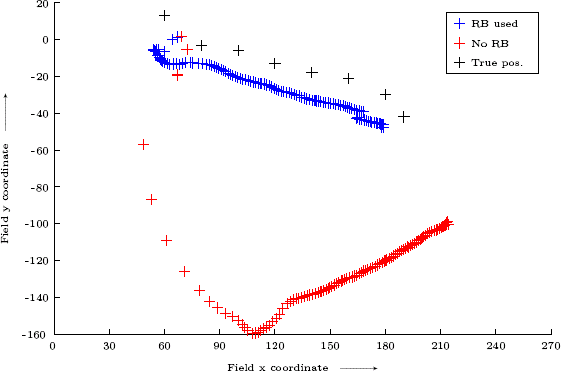
\includegraphics{rickfigs/florian.png} }
\end{center}
\caption{Comparison of ball localisation with and without using the
relative ball coordinate system. Truth data obtained manually from
video tape.}
\label{Fig:RelativeBallTest}
\end{figure}


\subsection{Incorporation and Tuning of Deadzones}
\label{locwm:deadzone}
The information content available to the EKF is very variable in
it's quality and `richness'. When there is insufficient information
available from which to determine the robot's own location
accurately, or more importantly, when the information available is
almost (but not quite) ambiguous, then we have noticed problems with
slow estimate `drift' with time. For example, we noticed that when
in the set state (just prior to kick-off), the head is typically fixed, staring at the ball, and it is quite possible for the robot to be only able to observe one or two objects on the field, and these from some distance away.

This resulted in the position estimates for the robot drifting
slowly away from the correct position. This `drift' is directly
analogous to a problem studied some time ago in parameter estimation
schemes in adaptive control (see for example
\cite{PetersenNarendra1982}). One of the schemes devised for
countering this drift was to use a `deadzone'
\cite{PetersenNarendra1982}, \cite{Middleton1988} in the estimation
part of the adaptive controller. We have therefore implemented this
in the EKF with code as follows:

\begin{alltt}
void KF::Deadzone(double* R, double* innovation, double CPC,
double eps) { 
  double invR;
  if ((eps<1.0e-08) || (CPC<1.0e-08) || (*R<1e-08))
  	return;
	if (ABS(*innovation)>eps) {
    invR=(ABS(*innovation)/eps-1)/CPC;
  } else {
    *innovation=0.0;
    invR=0.25/(eps*eps)-1.0/CPC;
  }
  if (invR<1.0e-08)
    invR=1e-08;
  if ( *R < 1.0/invR )
    *R=1.0/invR;
}
\end{alltt}

This function takes as inputs the current value of the measurement
covariance, $R$, the innovations $innovation$ (that is, deviation of
the predicted measurement from the observed measurement), the
variance of the predicted measurement $CPC$ and the size of the
deadzone, $eps$. The algorithm works by increasing the measurement
covariance, and in some cases adjusting the innovations used in the
actual EKF update. The rules used ensure that if the innovations are
smaller than the deadzone, then the EKF gives zero change to the
location estimates (by setting the innovations to zero) and also
adjusting the $R$ value used by the EKF.

\subsection{Implementation of Penalty Corner Objects}

The corner points of the penalty box have been identified by new
vision processing software. As a first step towards fulling
incorporating these objects into localisation, they were used for
goal keeper localisation in our 2006 code. Penalty corners were only
used when a valid background beacon could simultaneously be seen to
give a clear indication of which corner was being observed.
Incorporating these into keeper localisation proved to be a
substantial benefit to the quality of localisation observed.

\subsection{Other minor changes}
\label{locwm:other}
There were a number of changes to some of the constants used by the
EKF:
\begin{itemize}
  \item {Increase in the threshold for treating range measurements as outliers;}
  \item {Introduced an algorithm to ignore range measurements to goal objects or posts that are much
  larger than predicted. This proved particularly helpful for the
  goal keeper where occasional small size goals are recognised from
  within view of the keeper's own goal.}
  \item {Debugged the use of a sanity value to passed from vision, to alter the $R$ value for
  objects where there is some loss of confidence in the measurement accuracy. Specifically, if a goal
  post object is not contained entirely within the image, the uncertainty in the range to the goal post
  is increased significantly.}
  \item {We retuned the checks for EKF reset (`kidnapped robot') to make this occur less often.}
  \item {We removed `clipping' of the ball location, so that it is possible for the ball to be outside
  the field.}
\end{itemize}

The net result was that the ball velocity estimates were more
accurate and consistent; we believe we had a significant reduction
in occurrences of a `lost' goal keeper; and, our field players
mostly seemed to have sufficient accuracy in localisation to make
good behaviour decisions.
